% Every key fixes a sequence x^k_0, x^k_1, ... = TF_k(0), TF_k(1), ...
% Splitting takes an entry of a sequence as a new key; generating reads a
% sequence from its start as random bits. Same program as rng-key-tree.tex.
% Build: see figures/README.md
\documentclass[tikz, border = 6pt]{standalone}
\usepackage[T1]{fontenc}
\usepackage{lmodern}
\usepackage{amsmath}
\usetikzlibrary{calc}

\definecolor{hash}{HTML}{5B8C5A}
\definecolor{keep}{HTML}{2A7AB0}
\definecolor{fork}{HTML}{E08A2C}

\tikzset{
  cell/.style = {draw = white, line width = 1pt, minimum width = 13mm,
    minimum height = 6.5mm, inner sep = 0pt, font = \footnotesize},
  split/.style = {cell, fill = hash!35},
  gen/.style = {cell, fill = keep!30},
  unused/.style = {cell, fill = black!7, text = black!45},
  rowlabel/.style = {anchor = west, font = \small, inner sep = 1pt},
  note/.style = {anchor = west, font = \footnotesize, align = left, text = black!75},
  tree/.style = {black!45, line width = 0.5pt}
}

% column t of the table
\newcommand{\colx}[1]{3.9 + #1 * 1.32}

% \seqrow{row}{key in subscripts}{style of t = 0..5, comma separated}
\newcommand{\seqrow}[3]{%
  \foreach \s [count = \t from 0] in {#3} {
    \node[\s] at ({\colx{\t}}, -#1 * 0.8) {$x^{#2}_{\t}$};
  }
  \node[font = \small, text = black!45] at ({\colx{6}}, -#1 * 0.8) {$\cdots$};
}

\begin{document}
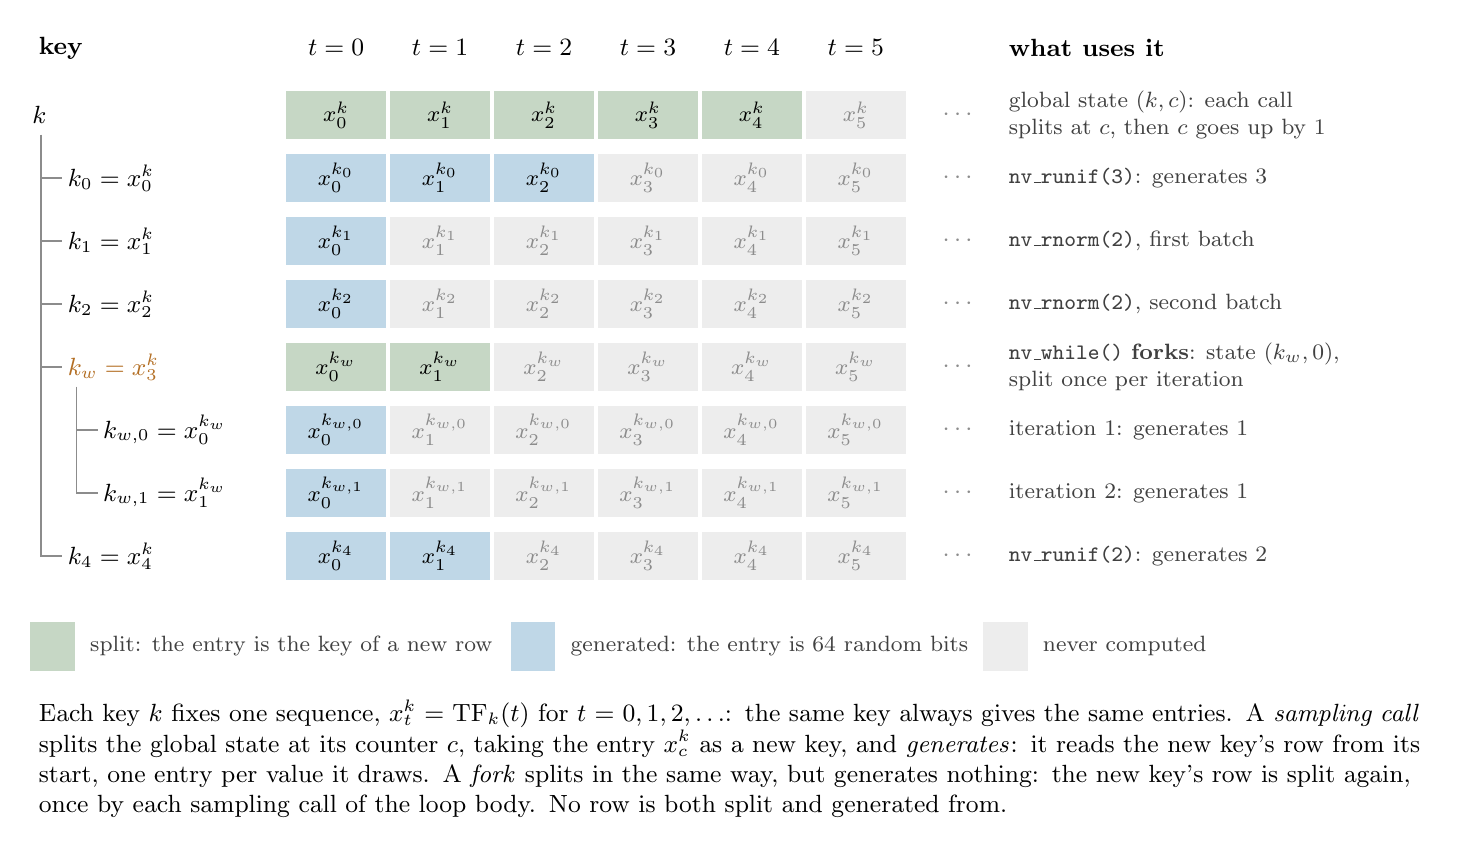
\begin{tikzpicture}

  % ---- header ---------------------------------------------------------------
  \node[anchor = west, font = \small\bfseries] at (0, 0.85) {key};
  \foreach \t in {0, ..., 5} {
    \node[font = \small] at ({\colx{\t}}, 0.85) {$t = \t$};
  }
  \node[note, font = \small\bfseries, text = black] at ({\colx{6} + 0.5}, 0.85) {what uses it};

  % ---- rows -------------------------------------------------------------------
  % row 0: the global key, only ever split, at the counters 0, ..., 4
  \node[rowlabel] at (0, 0) {$k$};
  \seqrow{0}{k}{split, split, split, split, split, unused}
  \node[note] at ({\colx{6} + 0.5}, 0) {global state $(k, c)$: each call\\splits at $c$, then $c$ goes up by 1};

  \node[rowlabel] at (0.45, -0.8) {$k_0 = x^k_0$};
  \seqrow{1}{k_0}{gen, gen, gen, unused, unused, unused}
  \node[note] at ({\colx{6} + 0.5}, -0.8) {\texttt{nv\_runif(3)}: generates 3};

  \node[rowlabel] at (0.45, -1.6) {$k_1 = x^k_1$};
  \seqrow{2}{k_1}{gen, unused, unused, unused, unused, unused}
  \node[note] at ({\colx{6} + 0.5}, -1.6) {\texttt{nv\_rnorm(2)}, first batch};

  \node[rowlabel] at (0.45, -2.4) {$k_2 = x^k_2$};
  \seqrow{3}{k_2}{gen, unused, unused, unused, unused, unused}
  \node[note] at ({\colx{6} + 0.5}, -2.4) {\texttt{nv\_rnorm(2)}, second batch};

  \node[rowlabel, text = fork!80!black] at (0.45, -3.2) {$k_w = x^k_3$};
  \seqrow{4}{k_w}{split, split, unused, unused, unused, unused}
  \node[note] at ({\colx{6} + 0.5}, -3.2) {\texttt{nv\_while()} \textbf{forks}: state $(k_w, 0)$,\\split once per iteration};

  \node[rowlabel] at (0.9, -4.0) {$k_{w,0} = x^{k_w}_0$};
  \seqrow{5}{k_{w,0}}{gen, unused, unused, unused, unused, unused}
  \node[note] at ({\colx{6} + 0.5}, -4.0) {iteration 1: generates 1};

  \node[rowlabel] at (0.9, -4.8) {$k_{w,1} = x^{k_w}_1$};
  \seqrow{6}{k_{w,1}}{gen, unused, unused, unused, unused, unused}
  \node[note] at ({\colx{6} + 0.5}, -4.8) {iteration 2: generates 1};

  \node[rowlabel] at (0.45, -5.6) {$k_4 = x^k_4$};
  \seqrow{7}{k_4}{gen, gen, unused, unused, unused, unused}
  \node[note] at ({\colx{6} + 0.5}, -5.6) {\texttt{nv\_runif(2)}: generates 2};

  % ---- the tree of keys -------------------------------------------------------
  \draw[tree] (0.15, -0.25) |- (0.42, -5.6);
  \foreach \y in {-0.8, -1.6, -2.4, -3.2} { \draw[tree] (0.15, \y) -- (0.42, \y); }
  \draw[tree] (0.6, -3.45) |- (0.87, -4.8);
  \draw[tree] (0.6, -4.0) -- (0.87, -4.0);

  % ---- legend -----------------------------------------------------------------
  \begin{scope}[shift = {(0, -6.75)}]
    \node[split, minimum width = 6mm] (l1) at (0.3, 0) {};
    \node[note, right = 1pt] at (l1.east) {split: the entry is the key of a new row};
    \node[gen, minimum width = 6mm] (l2) at (6.4, 0) {};
    \node[note, right = 1pt] at (l2.east) {generated: the entry is 64 random bits};
    \node[unused, minimum width = 6mm] (l3) at (12.4, 0) {};
    \node[note, right = 1pt] at (l3.east) {never computed};
  \end{scope}

  \node[anchor = north west, font = \small, align = left, text width = 17.6cm]
    at (0, -7.3) {%
    Each key $k$ fixes one sequence, $x^k_t = \mathrm{TF}_k(t)$ for $t = 0, 1, 2, \ldots$:
    the same key always gives the same entries.
    A \emph{sampling call} splits the global state at its counter $c$, taking the entry $x^k_c$
    as a new key, and \emph{generates}: it reads the new key's row from its start, one entry per
    value it draws.
    A \emph{fork} splits in the same way, but generates nothing: the new key's row is split again,
    once by each sampling call of the loop body.
    No row is both split and generated from.};

\end{tikzpicture}
\end{document}
